\subsection{Main Results: Complete MEDAGENT-X Pipeline}
\label{sec:main-results}

Experiment~6 evaluates the complete MEDAGENT-X workflow with the RAD-DINO predictor, training-only image-to-report retrieval, deterministic gray-zone fusion, the guarded label-fusion LLM, and the non-mutating evidence-verification LLM enabled. All configuration details, including the cohort, checkpoint, thresholds, retrieval parameters, LLM serving configuration, and Judge policy, are fixed as described in Section~4.1. The two LLMs are downstream review and verification components: neither is trained on the test set, and the evidence-verification LLM has no authority to modify a finalized diagnostic label.

\subsubsection{Study-Level Predictive Performance}

Table~\ref{tab:main-results} reports the final Experiment~6 outputs on the 906-study test cohort. The complete-test evaluation contains $10{,}872$ study--label cells, while the gray-zone analysis uses the fixed threshold-adjacent scope defined from the vision-only predictions. Under the Judge policy, a cell contributes to binary precision, recall, and F1 only when its CheXpert-derived ground truth is explicitly present or absent and the prediction is scoreable.

\begin{table}[H]
\centering
\caption{Main predictive results for Experiment~6, the complete MEDAGENT-X pipeline. Metrics are computed under the fixed Judge policy on the full test scope and the frozen gray-zone scope.}
\label{tab:main-results}
\resizebox{\columnwidth}{!}{%
\begin{tabular}{lrrrrrrr}
\toprule
Scope & Macro P & Macro R & Macro F1 & Micro P & Micro R & Micro F1 & Coverage \\
\midrule
Full test & 0.9117 & 0.6051 & 0.7246 & 0.9136 & 0.6195 & 0.7383 & 0.1492 \\
Gray zone & 0.8773 & 0.6950 & 0.7613 & 0.8824 & 0.7386 & 0.8041 & 0.1837 \\
\bottomrule
\end{tabular}%
}
\end{table}

On the full test set, the complete pipeline reaches a macro-F1 of $0.7246$ and a micro-F1 of $0.7383$. Relative to the vision-only baseline, this is an absolute improvement of $0.0275$ macro-F1 and $0.0341$ micro-F1. The improvement is primarily recall-oriented: macro recall increases from $0.5695$ to $0.6051$, while macro precision remains nearly unchanged, increasing from $0.9108$ to $0.9117$. This behavior is consistent with the intended operating regime of MEDAGENT-X: retrieved evidence is used to recover selected threshold-adjacent findings, rather than to replace the vision model or indiscriminately increase the number of positive predictions.

The effect is larger in the intervention scope. The gray-zone macro-F1 is $0.7613$ and the gray-zone micro-F1 is $0.8041$, compared with $0.6310$ and $0.6417$ for the vision-only gray-zone baseline. Gray-zone macro recall reaches $0.6950$ at macro precision $0.8773$. Thus, the largest change occurs exactly where the pipeline is permitted to act, while strong-zone predictions remain governed by the original vision-model decision.

\begin{figure}[H]
\centering
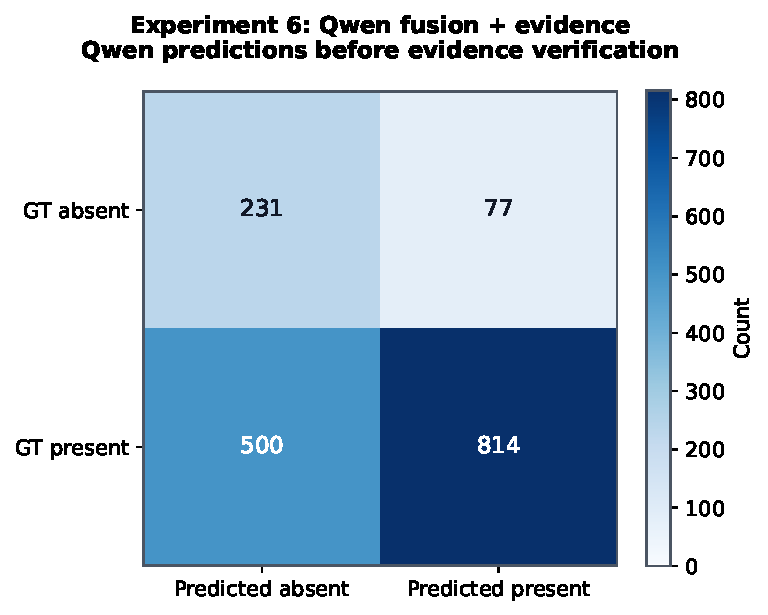
\includegraphics[width=0.82\columnwidth]{v2/experiments/visualizations_exp01_exp06/paper_figures/exp06_confusion_matrix.pdf}
\caption{Aggregate Judge-compatible confusion matrix for Experiment~6. The matrix contains only explicitly present and explicitly absent ground-truth cells with binary-scoreable predictions; uncertain and unmentioned ground-truth cells are excluded.}
\label{fig:main-confusion-matrix}
\end{figure}

Figure~\ref{fig:main-confusion-matrix} contains 814 true positives, 231 true negatives, 77 false positives, and 500 false negatives after aggregation across labels. The resulting positive precision is $814/(814+77)=0.9136$, and the positive recall is $814/(814+500)=0.6195$. The difference between these aggregate binary values and the macro values in Table~\ref{tab:main-results} is expected because macro metrics first compute each label's metric and then average across the 12 labels, whereas micro metrics pool the scoreable cells before computing the metric.

\subsubsection{Label-Wise Behavior and Continuous Discrimination}

The label-wise F1 values in Figure~\ref{fig:main-label-f1} show that performance is heterogeneous across the target findings. Lung Lesion and Lung Opacity attain the highest F1 values, $0.8348$ and $0.8074$, respectively. Consolidation, Pleural Effusion, Pneumonia, and Atelectasis are between $0.7397$ and $0.7517$. The most difficult labels are Pneumothorax and Enlarged Cardiomediastinum, with F1 values of $0.5930$ and $0.6078$. These differences reflect both visual difficulty and the uneven number of scoreable positive and negative examples available for each label; they motivate reporting macro metrics and per-label results rather than relying on a single pooled score.

\begin{figure}[H]
\centering
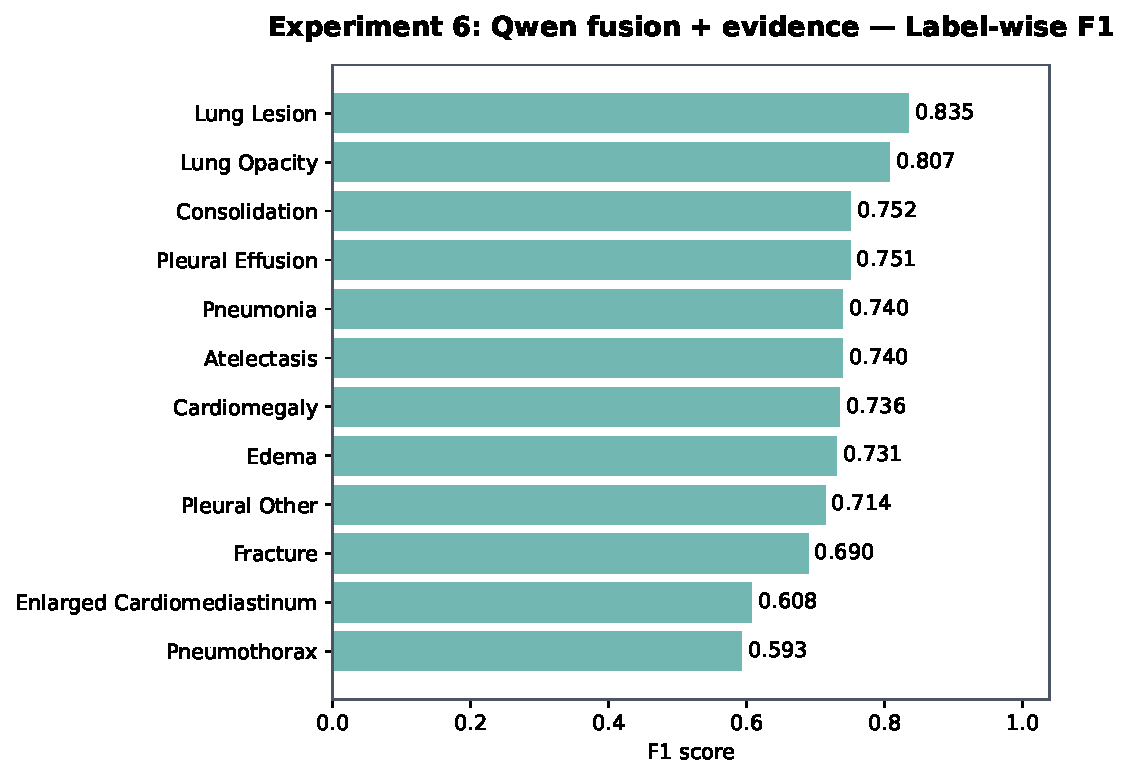
\includegraphics[width=\columnwidth]{v2/experiments/visualizations_exp01_exp06/paper_figures/exp06_label_f1.pdf}
\caption{Label-wise F1 scores for Experiment~6 on Judge-scoreable test cells. Evidence verification is non-mutating, so these are the finalized predictive labels produced after retrieval-grounded fusion.}
\label{fig:main-label-f1}
\end{figure}

The ROC and precision--recall plots provide a complementary view of the continuous RAD-DINO scores before hard-status fusion. They are not curves for the LLM outputs and do not treat the deterministic fusion transitions as continuous scores. The conventional curves in Figures~\ref{fig:main-roc} and~\ref{fig:main-pr} include all 12 labels and define the negative class as the union of absent, uncertain, and unmentioned ground-truth statuses. Under this formulation, the macro-AUROC is $0.7528$ and the macro average precision is $0.3276$. Label-wise AUROC ranges from $0.6930$ for Edema to $0.8306$ for Pneumothorax, while average precision ranges from $0.1477$ for Pneumonia to $0.5842$ for Pleural Effusion. This formulation is more representative of the complete multi-label test cohort, but it should not be confused with the stricter Judge-compatible binary evaluation because uncertain and unmentioned statuses are treated as negatives. Precision--recall curves are particularly informative in this imbalanced multi-label setting \cite{davis2006relationship}.

\begin{figure*}[t]
\centering
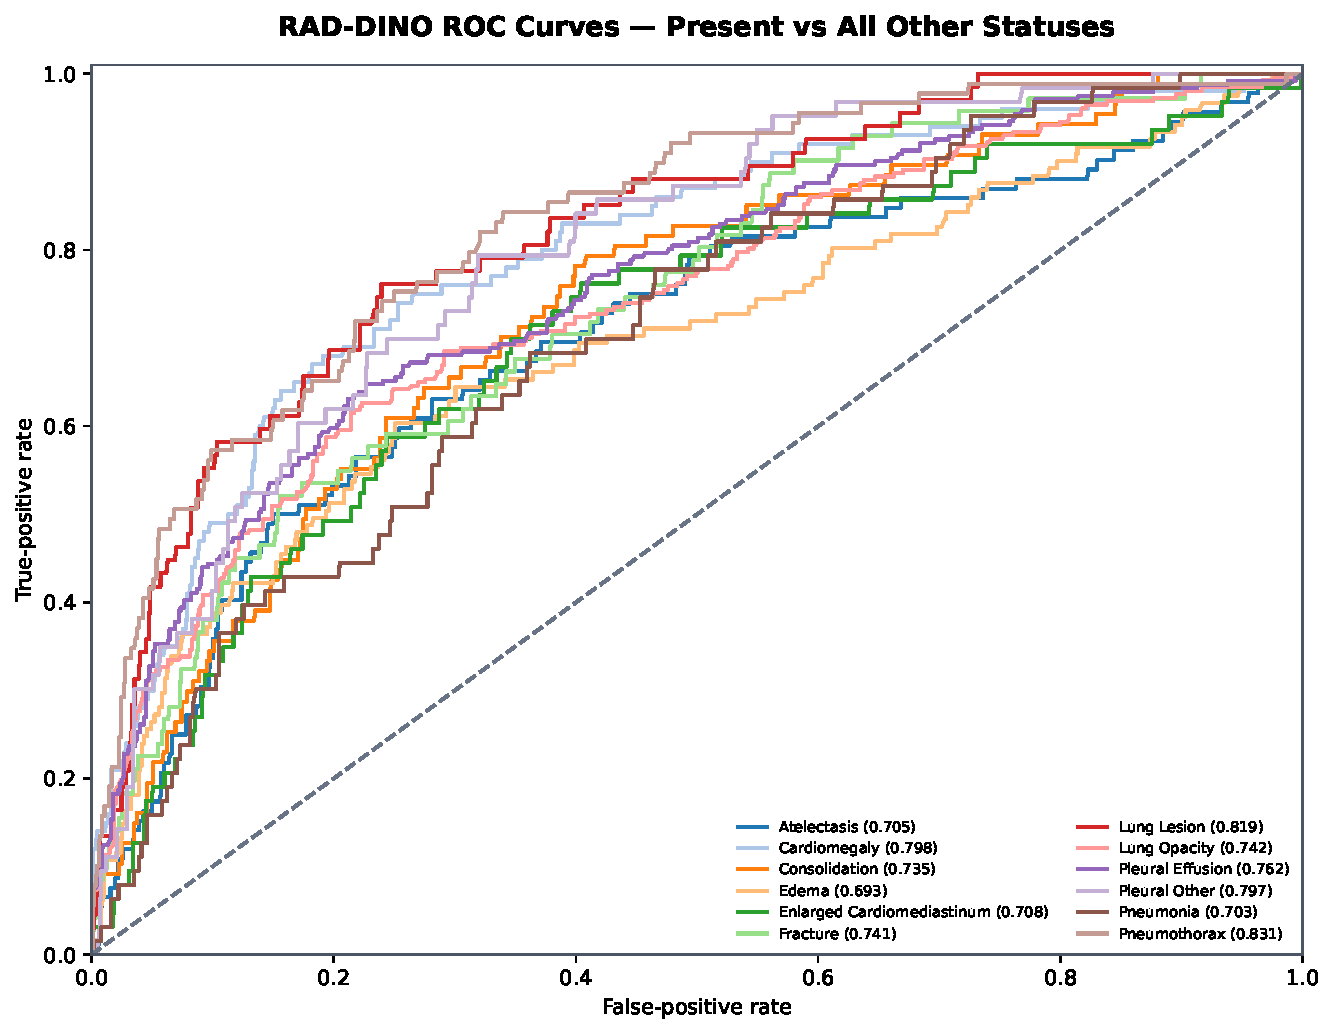
\includegraphics[width=0.92\textwidth]{v2/experiments/visualizations_exp01_exp06/07_roc_curves_present_vs_not_present.pdf}
\caption{RAD-DINO receiver-operating-characteristic curves using the conventional present-versus-not-present formulation. Absent, uncertain, and unmentioned ground-truth statuses are grouped as negative. The plot uses continuous vision probabilities and is therefore a discrimination analysis of the visual predictor, not an evaluation of hard-status LLM decisions.}
\label{fig:main-roc}
\end{figure*}

\begin{figure*}[t]
\centering
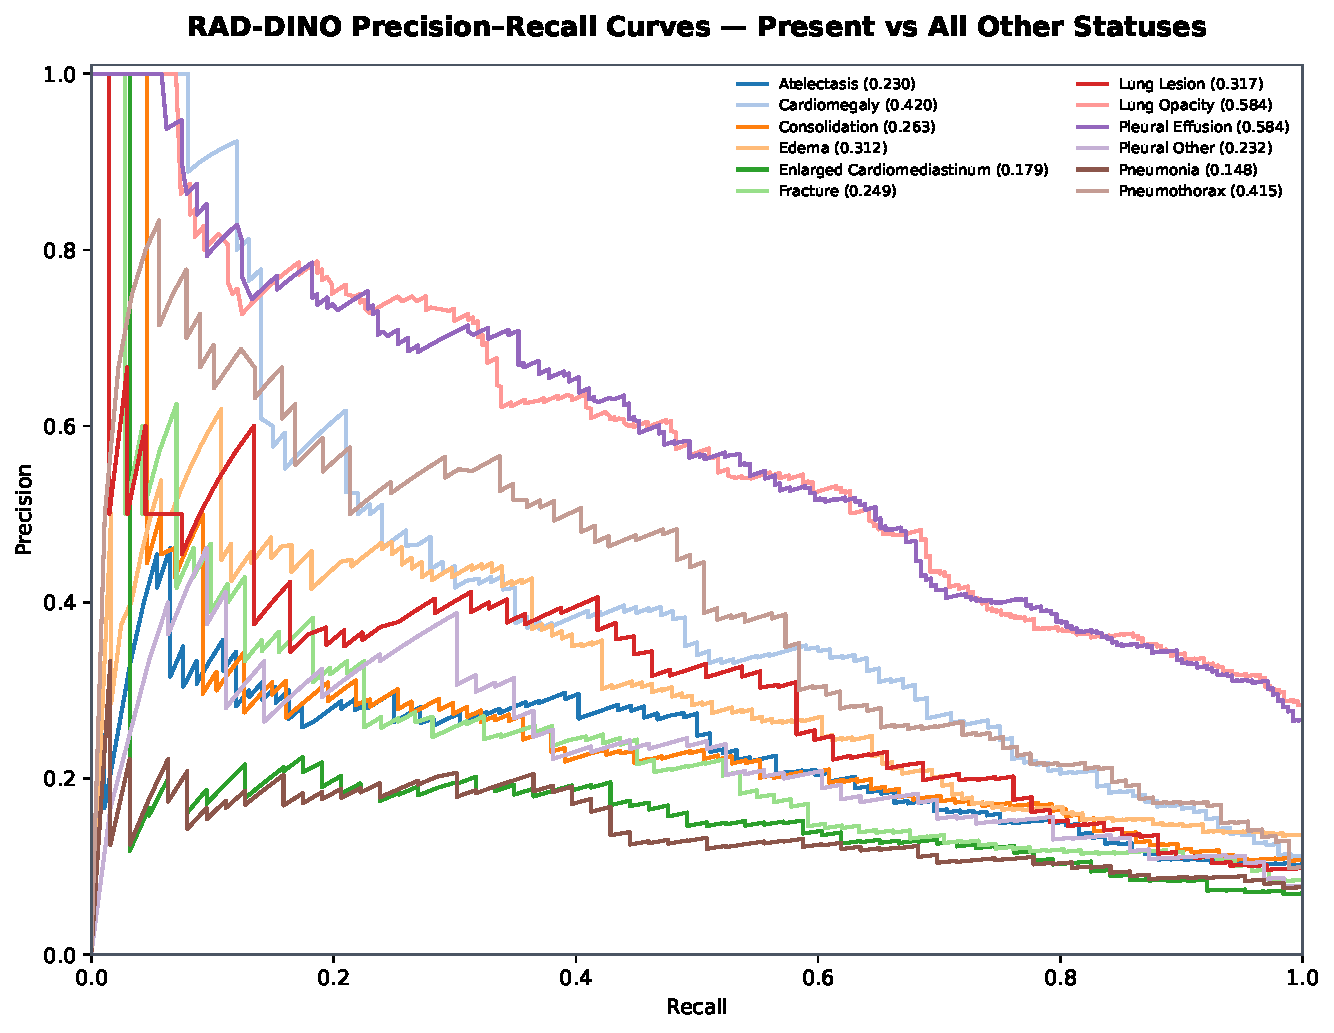
\includegraphics[width=0.92\textwidth]{v2/experiments/visualizations_exp01_exp06/08_pr_curves_present_vs_not_present.pdf}
\caption{RAD-DINO precision--recall curves under the conventional present-versus-not-present formulation across all 12 labels. Average precision is reported in the legend; the retrieval and LLM modules operate only after this continuous visual scoring stage.}
\label{fig:main-pr}
\end{figure*}

\subsubsection{Evidence Audit and Provenance}

The complete pipeline adds an audit layer to the predictive output. Across the 906 test studies, the evidence artifact contains 2,989 label-level evidence records. A total of 387 records correspond to labels whose final status differs from the vision-only status after the guarded fusion stage. The remaining records document unchanged predictions, including strong-zone labels and gray-zone labels for which the deterministic policy retained the vision status. Because the second LLM is non-mutating, these evidence records explain and qualify the final predictions without changing the predictive metrics in Table~\ref{tab:main-results}.

The study-level evidence-score distribution is reported in Table~\ref{tab:main-evidence-scores}. The 396 score-1 studies contain no final positive or uncertain supervised labels and therefore require no label-level evidence review. Among the 510 studies with at least one evidence-bearing prediction, 425 ($83.3\%$) receive an overall score of 4 or 5. These scores are audit outputs, not ground-truth diagnostic labels and not substitutes for the Judge metrics.

\begin{table}[H]
\centering
\caption{Study-level evidence scores for Experiment~6 across the 906-study test cohort.}
\label{tab:main-evidence-scores}
\begin{tabular}{lrr}
\toprule
Evidence score & Studies & Share \\
\midrule
1 & 396 & 43.7\% \\
2 & 15  & 1.7\% \\
3 & 70  & 7.7\% \\
4 & 420 & 46.4\% \\
5 & 5   & 0.6\% \\
\midrule
Total & 906 & 100.0\% \\
\bottomrule
\end{tabular}
\end{table}

To make the audit output concrete, Figure~\ref{fig:main-evidence-json} shows an excerpt from a persisted, schema-validated Experiment~6 evidence record. The record links the final label status to the vision status, retrieved support counts, an evidence score, an assessment, cited de-identified cases, and a natural-language rationale. The excerpt is shortened to one label-level record for readability; the complete JSON artifact retains all predicted labels and evidence fields.

\begin{figure}[H]
\centering
\begin{minipage}{\columnwidth}
\scriptsize
\begin{verbatim}
{
  "study_key": "patient00877/study1",
  "verification_policy_version":
    "llm_evidence_verification_review_v1",
  "overall_evidence_score": 4,
  "label_evidence_details": [{
    "label": "Atelectasis",
    "fused_status": "present",
    "vision_status": "present",
    "evidence_score": 4,
    "retrieval_support": "strong",
    "retrieval_positive_count": 13,
    "retrieval_negative_count": 0,
    "contradiction_level": "none",
    "fusion_changed": false,
    "evidence_summary": "Strong retrieval evidence (13/13 positive mentions) aligns with vision findings. No conflicting evidence identified.",
    "supporting_evidence": [{
      "case_id": "patient51142/study4",
      "similarity": 0.37341630458831787,
      "snippet": "decreased lung volumes with bibasilar opacities, likely atelectasis"
    }]
  }]
}
\end{verbatim}
\end{minipage}
\caption{Excerpt from an actual schema-validated Experiment~6 evidence-verification record. The study and case identifiers are de-identified. Long strings and the remaining label records are omitted only for presentation.}
\label{fig:main-evidence-json}
\end{figure}

\begin{figure}[H]
\centering
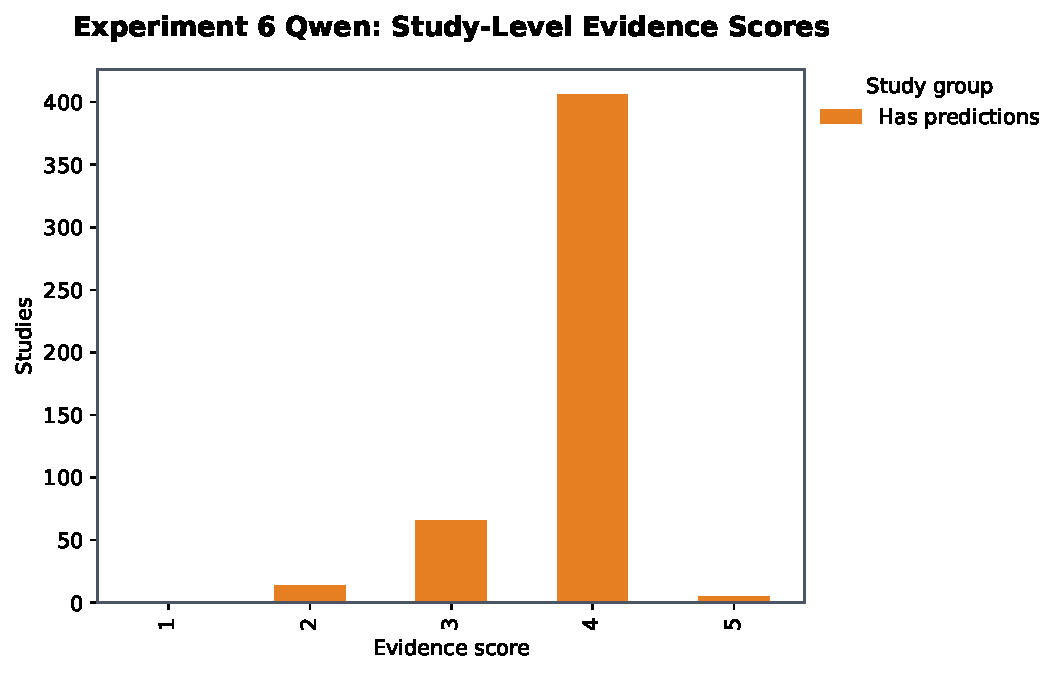
\includegraphics[width=\columnwidth]{v2/experiments/visualizations_exp01_exp06/paper_figures/exp06_qwen_evidence_study_score_distribution.pdf}
\caption{Study-level evidence scores for Experiment~6. Score 1 is assigned to studies with no final positive or uncertain supervised prediction; scores 2--5 summarize evidence for studies with at least one evidence-bearing prediction.}
\label{fig:main-evidence-study-scores}
\end{figure}

At the label level, retrieved reports provide strong support for 1,303 records, moderate support for 903, weak support for 231, and no support for 523. A further 13 records are classified as mixed and 16 as contradictory. The support distribution is label-dependent: Atelectasis, Edema, Pleural Effusion, and Consolidation have the largest proportions of strong support, whereas Enlarged Cardiomediastinum has little positive retrieval support and a large no-support component. This pattern is consistent with the constrained design: the system records weak or contradictory retrieval evidence rather than converting it automatically into a positive diagnosis.

\begin{figure}[H]
\centering
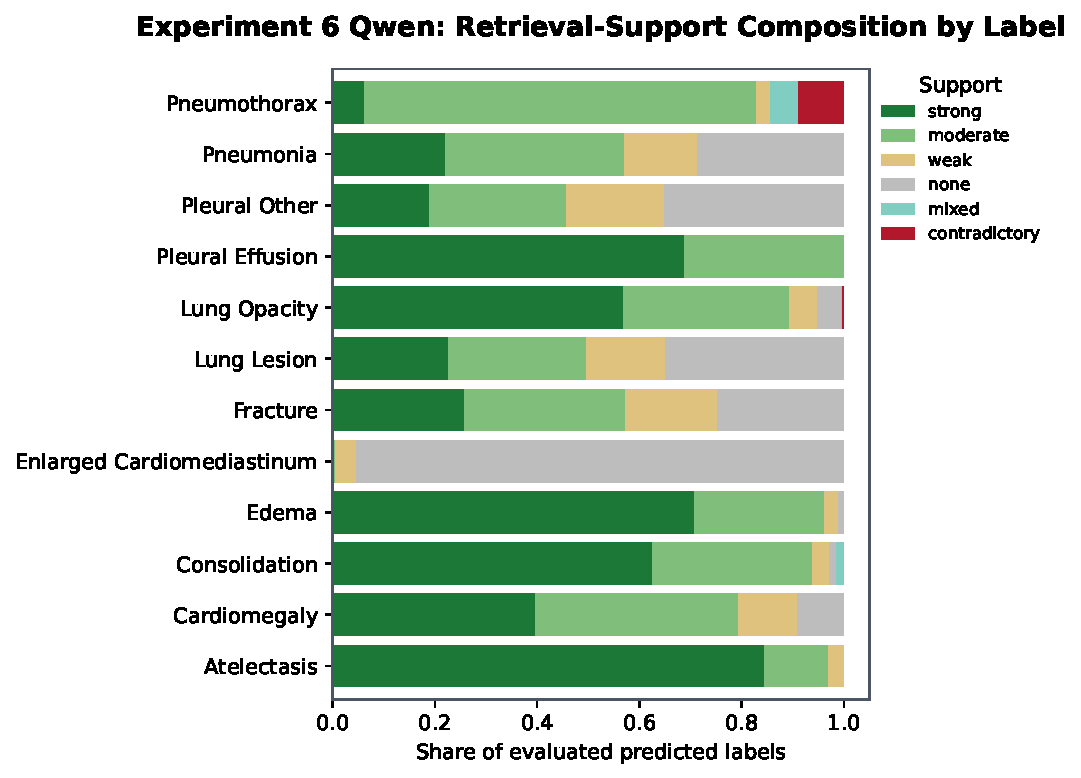
\includegraphics[width=\columnwidth]{v2/experiments/visualizations_exp01_exp06/paper_figures/exp06_qwen_evidence_retrieval_support_by_label.pdf}
\caption{Composition of retrieval-support assessments for evidence-bearing label records in Experiment~6. Support categories describe the retrieved report context and are separate from the frozen CheXpert-derived ground truth.}
\label{fig:main-evidence-support}
\end{figure}

Figure~\ref{fig:main-evidence-changed} compares evidence scores for fusion-changed and unchanged labels. Changed labels are concentrated in the moderate-to-high evidence categories, but the figure also shows that not every evidence-bearing record is a gray-zone intervention. This distinction is important for auditability: the pipeline preserves evidence for both decisions it changed and decisions it retained, enabling a reviewer to distinguish the reason for an intervention from the evidence associated with an unchanged prediction.

\begin{figure}[H]
\centering
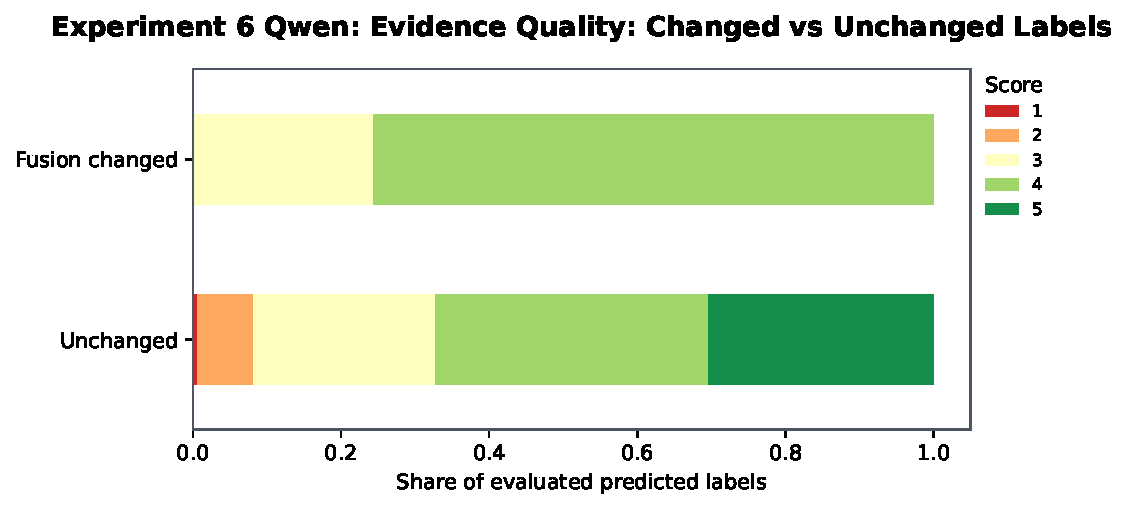
\includegraphics[width=\columnwidth]{v2/experiments/visualizations_exp01_exp06/paper_figures/exp06_qwen_evidence_changed_vs_unchanged.pdf}
\caption{Evidence-score composition for fusion-changed and unchanged label records in Experiment~6. The second LLM reports evidence quality but cannot edit either group.}
\label{fig:main-evidence-changed}
\end{figure}

The persisted evidence checkpoint contains 491 records produced by the LLM evidence-verification policy and 415 records produced by the deterministic verification policy. This is a provenance property of the saved run rather than a randomized comparison between verification methods. Accordingly, Figures~\ref{fig:main-evidence-study-scores}--\ref{fig:main-evidence-changed} are interpreted descriptively: they characterize the evidence and fallback behavior emitted by the complete pipeline, while the predictive claims remain based on the fixed Judge evaluation of the final labels.

\begin{figure}[H]
\centering
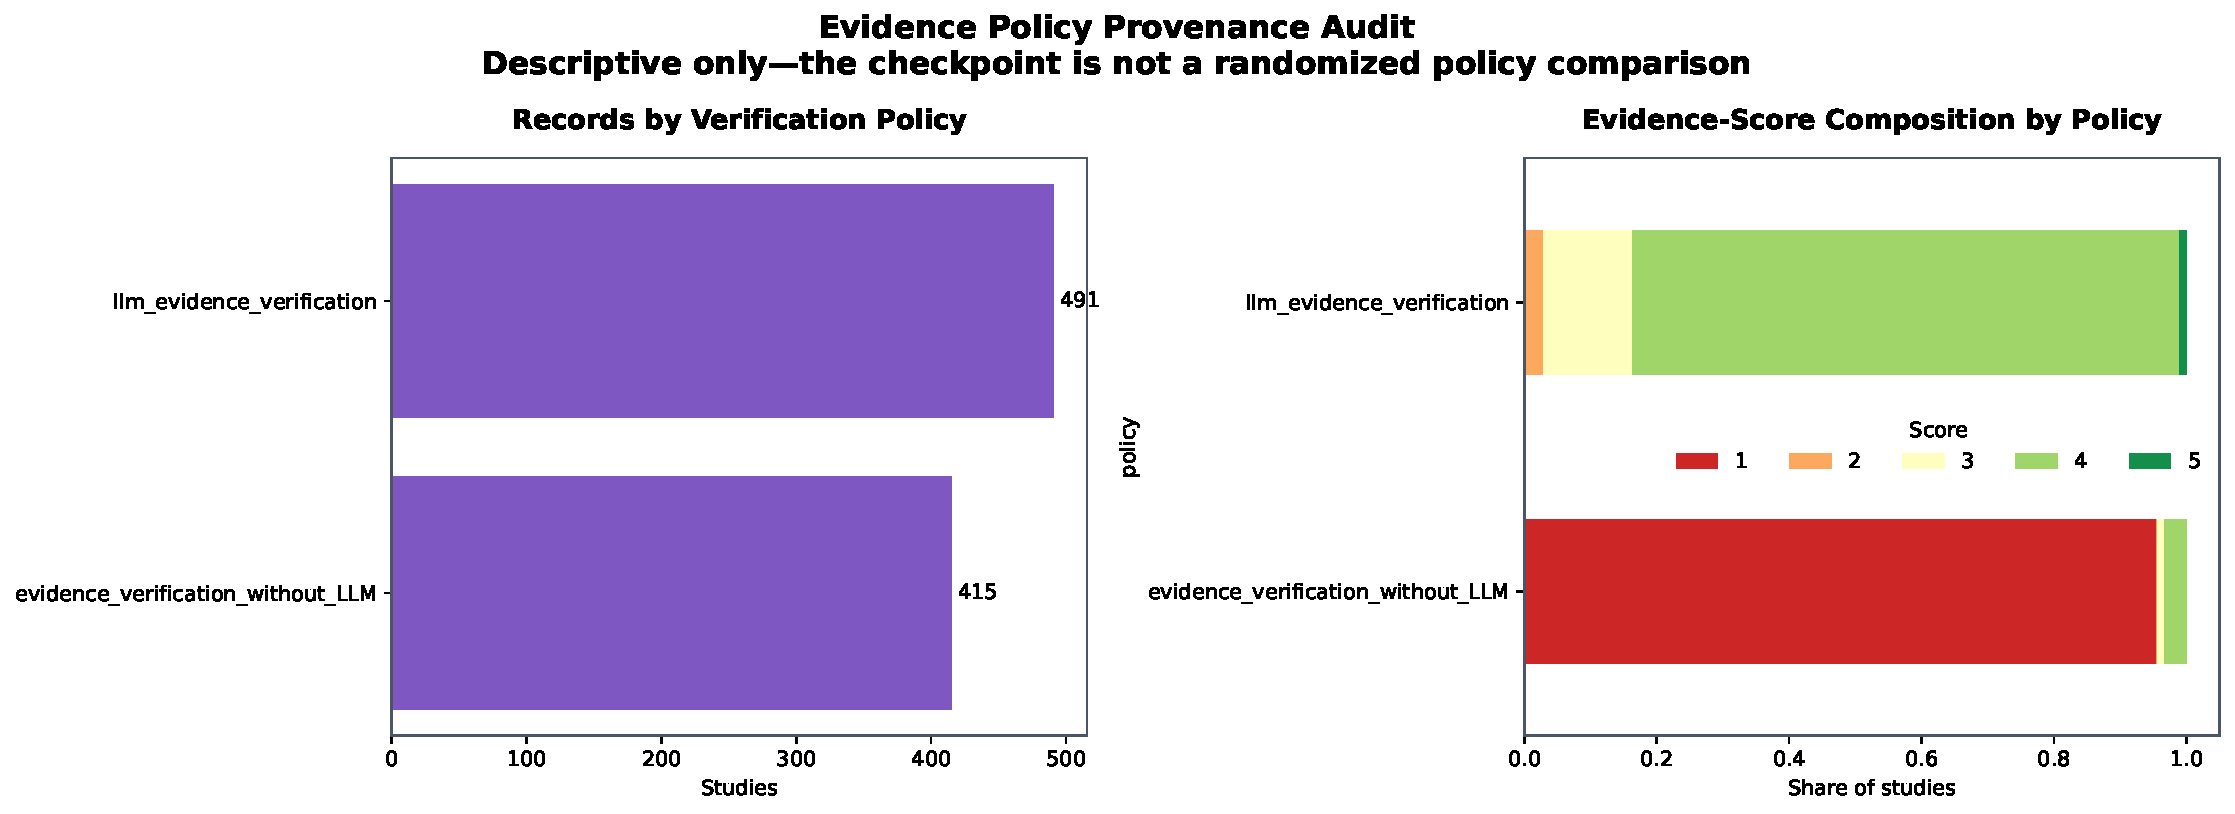
\includegraphics[width=\columnwidth]{v2/experiments/visualizations_exp01_exp06/11_evidence_policy_provenance.pdf}
\caption{Verification-policy provenance for the saved Experiment~6 evidence artifact. The mixture of LLM and deterministic records is shown for transparency; this plot is not a head-to-head policy comparison.}
\label{fig:main-evidence-provenance}
\end{figure}

Taken together, Experiment~6 demonstrates the intended separation of responsibilities. RAD-DINO supplies the primary visual probabilities, deterministic retrieval-grounded fusion makes the limited gray-zone label transitions, and the two LLM roles provide constrained review and evidence characterization. The measurable predictive gain is concentrated in recall and F1, while the principal contribution of the second LLM is the addition of study--label-level evidence and provenance without granting the language model diagnostic authority.
